\section{Introduction}
\label{sec:introduction}

As conversational Large Language Models (LLMs) are increasingly integrated into customer support, clinical workflows, legal analysis, and autonomous agent loops, verifying that chatbot outputs adhere to safety standards is a paramount operational requirement. While human moderation remains the authoritative gold standard, manual auditing cannot scale to the throughput demands of continuous production monitoring. Consequently, automated evaluation pipelines—popularized under the \textit{LLM-as-a-judge} paradigm~\cite{chiang2023vicuna,zheng2023judging,wang2023pandalm}—are widely adopted to evaluate conversational responses and detect safety violations~\cite{zhang2024safetybench,mazeika2024harmbench}.

Standard LLM-as-a-judge deployments rely almost exclusively on commercial cloud-hosted frontier models or large open-weight clusters ($70\text{B}+$ parameters)~\cite{touvron2023llama,tan2025judgebench,bavaresco2025llms}. While effective for high-level capabilities, this centralized cloud paradigm introduces persistent operational and governance challenges:
\begin{enumerate}
    \item \textbf{Data Privacy and Regulatory Governance:} While lawful cloud processing can be structured through formal Data Processing Agreements (DPAs) and institutional safeguards, transmitting user conversations to external commercial inference APIs introduces ongoing compliance management under data protection frameworks such as GDPR and HIPAA~\cite{debenedetti2024evading}. Local model inference avoids sending evaluated dialogue data to third-party model APIs, ensuring conversational data remains within internal boundaries, though institutional regulatory compliance ultimately depends on broader system-level security controls.
    \item \textbf{Economic and Throughput Overhead:} Sustained offline evaluation of high-volume conversational logs incurs recurring API token expenditures and operational exposure to rate-limiting bottlenecks.
    \item \textbf{Logit Obfuscation and Uncertainty Blindness:} Commercial model APIs frequently restrict or withhold raw next-token logit distributions, preventing downstream systems from extracting continuous probability estimates or evaluating predictive confidence.
\end{enumerate}

These operational constraints motivate investigating \textit{small open-weight language models} (SLMs) with fewer than 2 billion parameters~\cite{yang2024qwen25,allal2025smollm2} as localized safety evaluators. Sub-2B models can execute deterministically on commodity x86 CPUs within bounded memory footprints ($\le 8\text{ GB}$ system RAM, peak resident set size $< 1.2\text{ GB}$), enabling self-contained on-premises evaluation without requiring dedicated GPU acceleration.

\begin{figure}[t]
    \centering
    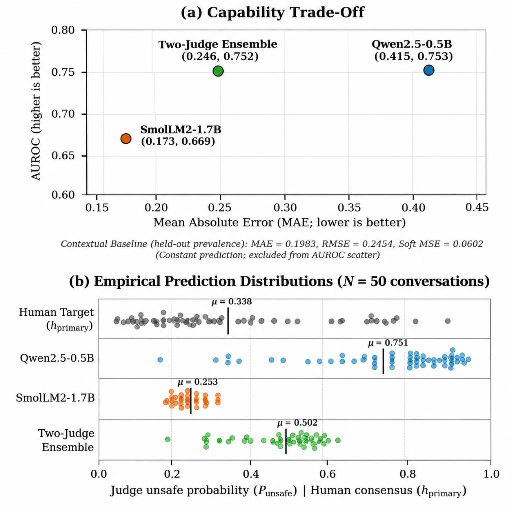
\includegraphics[width=\columnwidth]{figures/fig1_tradeoff.pdf}
    \caption{Evaluator polarization and the ensembling trade-off frontier on an exploratory sample of $N=50$ multi-turn adversarial conversations from Google DICES-350. (a) Capability trade-off plane: Mean Absolute Error (MAE, lower is better) versus majority-consensus discrimination ($\text{AUROC}$, higher is better). Qwen2.5-0.5B achieves high ranking sensitivity ($\text{AUROC} = 0.7529$, Spearman $\rho = 0.5680$) but high error ($\text{MAE} = 0.4152$). SmolLM2-1.7B achieves the lowest judge MAE ($0.1734$) but compressed ranking acuity ($\text{AUROC} = 0.6690, \rho = 0.3929$). The Two-Judge Ensemble provides an empirical compromise, cutting Qwen's MAE by $40.6\%$ while capturing the highest rank correlation ($\rho = \mathbf{0.5903}$) and preserving AUROC ($0.7517$). The ensemble does not universally dominate: SmolLM2 achieves lower sample MAE, and a 5-fold held-out prevalence baseline achieves lower squared error ($\text{Soft MSE} = 0.0602$). (b) Single-model prediction distributions ($N=50$) demonstrating Qwen's positive hazard bias ($\mu = 0.751$) and SmolLM2's variance collapse ($\sigma = 0.039$) clustered near dataset prevalence ($0.338$).}
    \label{fig:tradeoff}
\end{figure}

However, deploying compact models as autonomous safety evaluators introduces documented reliability risks. Constrained parameter capacities make small models prone to inductive biases, severe probability miscalibration, and vulnerability to subtle phrasing shifts~\cite{tan2025judgebench,schwinn2026coin}. Recent audits demonstrate that automated judges can collapse toward chance-level accuracy when evaluating adversarial distributions~\cite{schwinn2026coin}. Furthermore, existing benchmarks predominantly collapse multi-rater evaluations into binary majority consensus, obscuring the nuanced distribution of human judgments~\cite{aroyo2023dices,davani2022dealing,rottger2022two}.

In classical machine learning, ensembling diverse model checkpoints is a recognized approach to mitigate individual inductive biases and improve predictive reliability~\cite{lakshminarayanan2017simple,ovadia2019can}. While multi-agent jury architectures have been explored for frontier models~\cite{verga2024replacing,qian2026who}, whether an ensemble of \textit{heterogeneous sub-2B open-weight models} running locally on commodity CPUs can reliably approximate continuous human safety consensus remains fundamentally uncharacterized.

To investigate this question, this paper presents \textbf{TrustEval}, an empirical study evaluating the representational accuracy, ranking discrimination, calibration behaviour, and error-uncertainty dynamics of small open-weight LLM safety judges. We analyze an equal-weight ensemble of two structurally distinct sub-2B models—\texttt{Qwen2.5-0.5B-Instruct} (0.49B parameters) and \texttt{SmolLM2-1.7B-Instruct} (1.71B parameters)—evaluated on multi-turn conversational dialogues drawn from the Google DICES-350 benchmark~\cite{aroyo2023dices}. Each conversation in DICES-350 contains ratings from 104 retained human crowd annotators, allowing us to evaluate models directly against continuous human consensus proportions ($h_{\text{primary}} \in [0, 1]$). Furthermore, we examine whether inter-judge disagreement ($\Delta = |P_{\text{qwen}} - P_{\text{smol}}|$) functions as an exploratory candidate correlate for ensemble evaluation error.

As previewed in Fig.~\ref{fig:tradeoff}, our empirical investigation uncovers a pronounced trade-off between constituent judges: Qwen2.5-0.5B exhibits strong discriminative hazard ordering alongside severe positive prediction bias, whereas SmolLM2-1.7B achieves low absolute error through conservative prevalence anchoring at the cost of compressed prediction variance. An unweighted ensemble negotiates this trade-off frontier, moderating prediction error relative to Qwen while improving rank correlation over both individual judges.

\subsection{Research Questions}
\label{sec:rqs}

This paper addresses three research questions established in our pre-registered experimental protocol:
\begin{itemize}
    \item \textbf{RQ1 (Representation and Point Error):} Can small open-weight LLMs ($\le 1.7\text{B}$ parameters) running on commodity CPU hardware approximate continuous human safety consensus ($h \in [0, 1]$), and how does an equal-weight ensemble compare against individual constituent judges and naive prevalence baselines in point error (MAE, RMSE, Soft MSE) and decile calibration (Soft ECE-10)?
    \item \textbf{RQ2 (Discriminative Ranking Capacity):} How do individual small judges and their ensemble perform in ranking conversational hazard relative to human consensus (Pearson $r$, Spearman $\rho$, AUROC), and does ensembling preserve discriminative sensitivity while tempering single-model prediction bias?
    \item \textbf{RQ3 (Disagreement as a Candidate Error Correlate):} Does inter-judge disagreement ($\Delta$) between diverse small judges provide a statistically defensible, cross-validated candidate surrogate signal for ensemble evaluation error, predicting uncertainty beyond response character length and ensemble predicted unsafe probability?
\end{itemize}

\subsection{Summary of Contributions}
\label{sec:contributions}

The primary contributions of this paper are:
\begin{enumerate}
    \item \textbf{Empirical Audit of Sub-2B Judges on Continuous Human Consensus:} We conduct an empirical evaluation of sub-2B open-weight LLMs tasked with predicting continuous human safety consensus ($h_{\text{primary}} \in [0, 1]$) derived from 104 crowd annotators per item ($5,200$ total ratings) across 50 multi-turn dialogues sampled from Google DICES-350.
    \item \textbf{Characterization of Single-Judge Trade-Offs:} We identify a clear divergence in small-model evaluation behaviour: Qwen2.5-0.5B achieves high discriminative ordering ($\text{AUROC} = 0.7529, \text{Spearman } \rho = 0.5680$) but exhibits substantial positive prediction bias ($\mu = 0.7513$ vs. human mean $0.3381$) and miscalibration ($\text{ECE-10} = 0.4128$). Conversely, SmolLM2-1.7B achieves the lowest observed sample MAE ($0.1734$) via variance compression ($\sigma = 0.0388$) near sample prevalence, with modest binary discrimination ($\text{AUROC} = 0.6690$) and a positive rank correlation ($\rho = 0.3929, p = 0.0048$). We document that SmolLM2's MAE advantage is test-sensitive (statistically significant under a paired $t$-test and sign test, but non-significant under a Wilcoxon signed-rank test after family-wise Holm adjustment; $W = 427.0, p_{\text{adj}} = 0.0843$).
    \item \textbf{Empirical Pareto Expansion via Ensembling:} We show that an equal-weight two-judge ensemble synthesizes these complementary behaviours, cutting Qwen's MAE by $40.6\%$ (to $0.2464$, $p = 1.04 \times 10^{-7}$) and Soft MSE by $67.6\%$ ($p = 2.85 \times 10^{-9}$) while maintaining comparable AUROC ($0.7517$) and attaining the highest rank correlation ($\rho = \mathbf{0.5903}$, $p = 6.43 \times 10^{-6}$) and linear correlation ($r = \mathbf{0.4992}$, $p = 0.0002$) across all evaluators. We emphasize that ensembling represents an observed empirical trade-off rather than universal superiority: it does not outperform SmolLM2 in point MAE, and it moderates rather than completely eliminates prediction bias.
    \item \textbf{Empirical Baseline Reality Check:} We transparently document that in squared error (Soft MSE), a naive 5-fold held-out prevalence baseline achieves the lowest overall error ($0.0602$), outperforming all evaluated models including the ensemble ($0.0713$), illustrating the challenge small models encounter under quadratic loss when competing against sample prevalence.
    \item \textbf{Exploratory Analysis of Disagreement as an Error Correlate:} We show that inter-judge disagreement ($\Delta$) exhibits a nominally significant positive association with ensemble absolute error ($r = 0.3125, p = 0.0271$). In nested in-sample OLS regression controlling for response length and ensemble prediction, adding $\Delta$ yields a statistically significant incremental variance gain ($F(1, 46) = 5.676, p = 0.0214$) and an out-of-fold descriptive gain of $\Delta R^2_{\text{OOF}} = +0.0805$ across 5-fold cross-validation. We rigorously qualify disagreement as a preliminary candidate correlate rather than a validated uncertainty metric.
    \item \textbf{Practical Edge-Inference Profiling:} We demonstrate that deterministic next-token logit scoring executes locally on commodity x86 laptop CPUs within a bounded envelope ($< 1.2\text{ GB}$ peak resident set size), confirming the computational feasibility of decentralized safety auditing.
\end{enumerate}

\subsection{Paper Roadmap}
\label{sec:roadmap}

The remainder of this paper is organized as follows: Section~\ref{sec:related_work} synthesizes related literature across LLM judges, safety benchmarks, calibration, and ensemble uncertainty. Section~\ref{sec:dataset_ground_truth} details the DICES-350 benchmark, crowd annotator filtering, and continuous target formulation. Section~\ref{sec:methodology_experimental_setup} outlines model architectures, native ChatML prompt serialization, and logit scoring protocols. Section~\ref{sec:results} presents empirical findings across point error, calibration, discriminative ranking, and inter-judge disagreement modeling (Subsection~\ref{subsec:disagreement_analysis}). Section~\ref{sec:discussion} discusses operational trade-offs, calibration nuances, and edge deployment implications. Section~\ref{sec:limitations_ethics} details empirical limitations and responsible AI considerations. Finally, Section~\ref{sec:conclusion} concludes the paper with future research directions.
